
\section{Site inleiding}\label{siteinleiding}
Dimpact is gebouwd met het CMS(Content Management System) \emph{Drupal}. De huidige versie is \emph{Drupal 7.23}.
Drupal is geschreven in de programmeertaal \emph{PHP}.

Bekijk de volgende websites voor uitgebreide informatie en naslagwerk:

\begin{enumerate}
\item \url{http://drupal.org}
\item \url{http://www.drupalin24dagen.nl/}
\item \url{http://www.drupalhandboek.nl/}
\end{enumerate}


\subsection{Voorpagina}\label{voorpagina}

\subsubsection{Grid}

De template van de website bestaat uit een grid, een soort geraamte. Het grid is opgebouwd uit verschillende regio's. In elke regio kunnen blokken geplaatst worden. In de paragraaf \emph{Felix}\seeone{felix} staat beschreven hoe en welke je blokken kunt toevoegen aan een regio. 

\bigskip

\begin{center}
	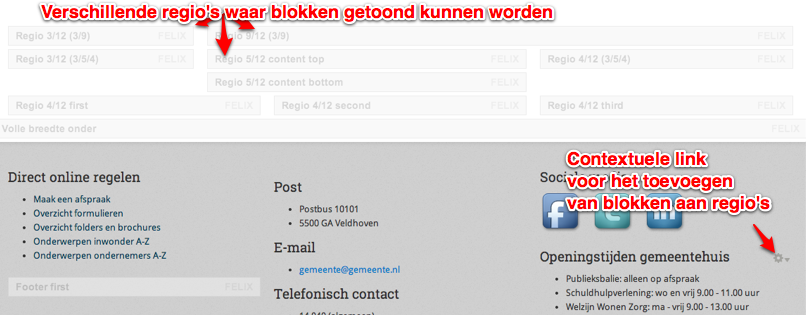
\includegraphics[width=\textwidth]{img/grid1.png}
\end{center}

\subsubsection{Blokken}

In het onderstaande afbeelding worden alle bestaande blokken op voorpagina in het kort toegelicht.

\bigskip

\begin{center}
	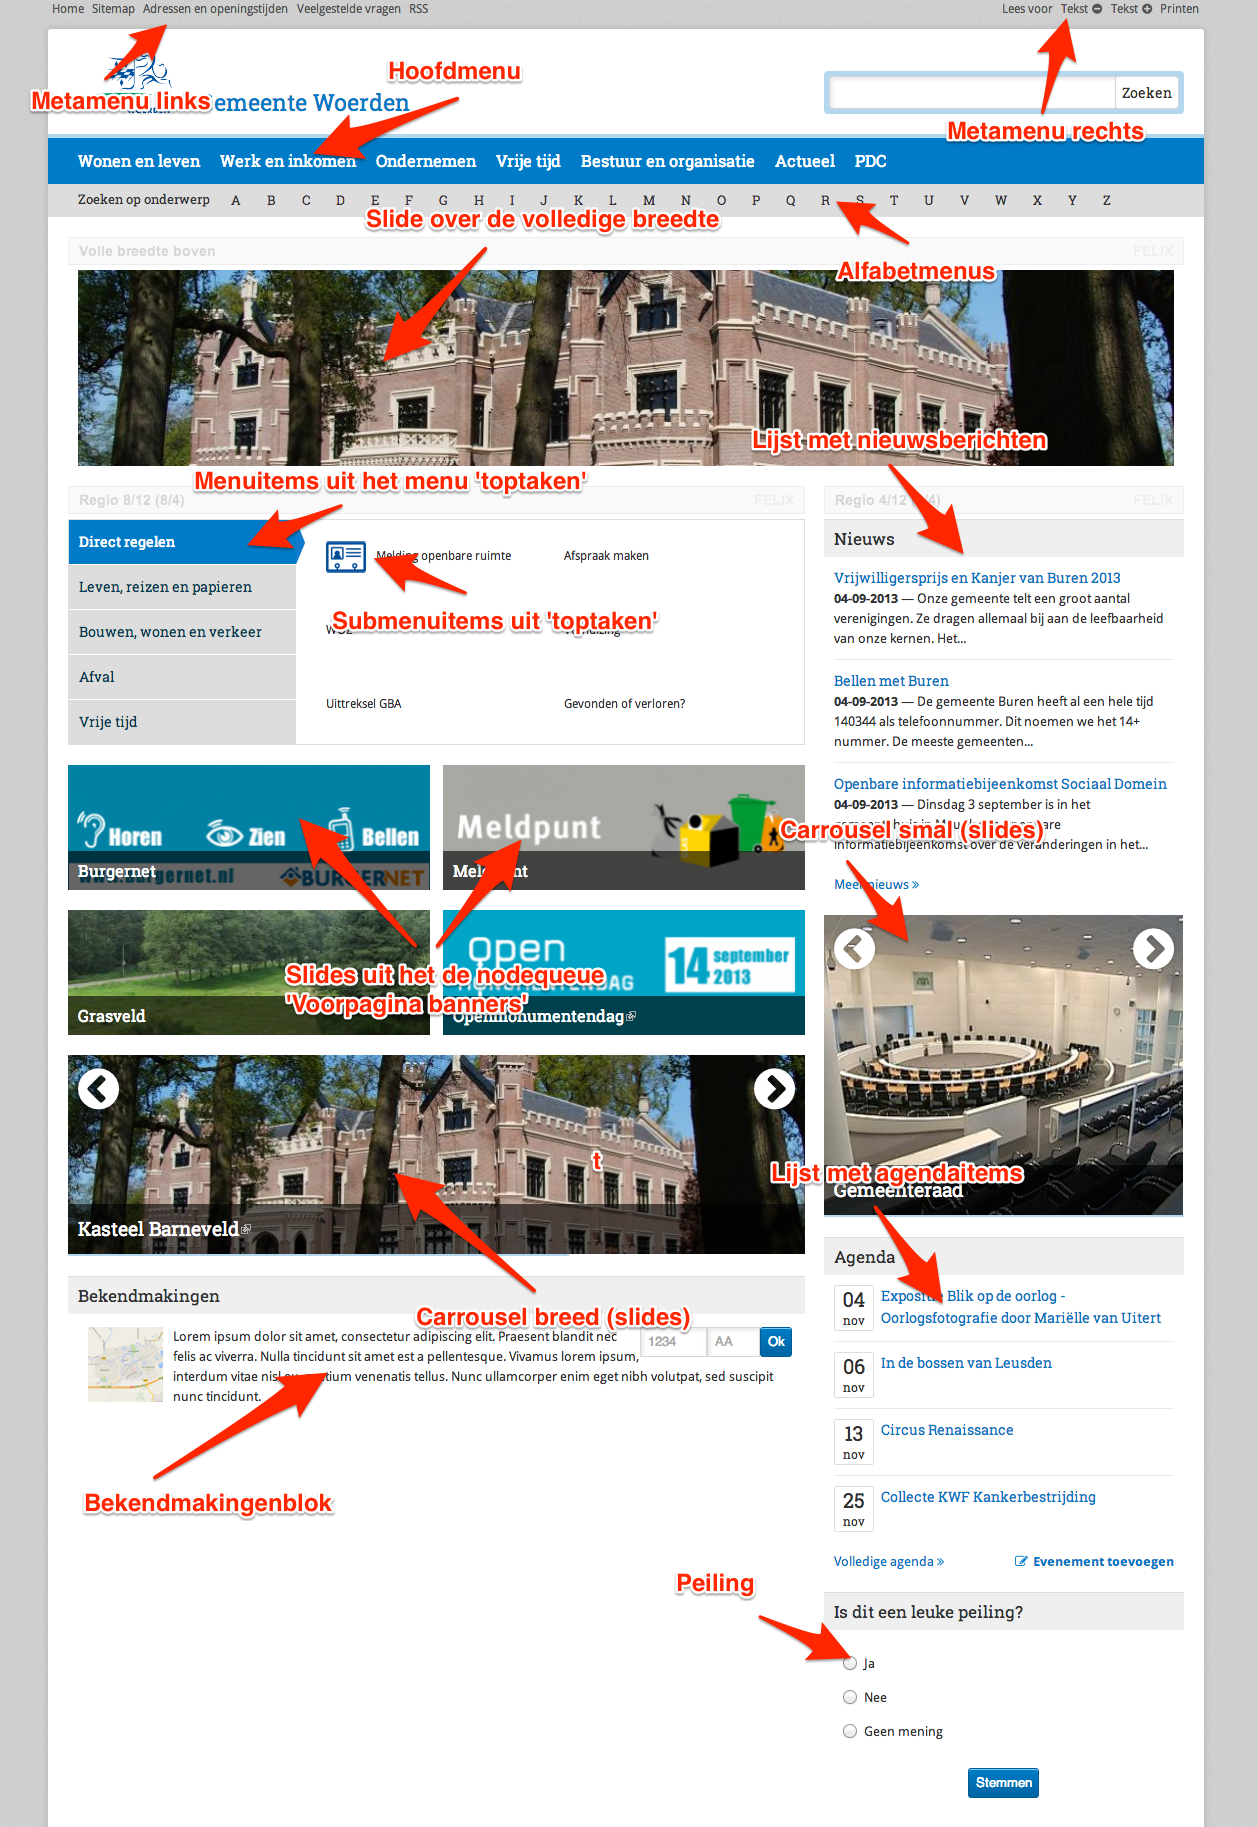
\includegraphics[width=\textwidth]{img/voorpagina.png}
\end{center}

\subsubsection{Footer}

In het onderstaande afbeelding worden alle bestaande blokken in de footer in het kort toegelicht. De footer bestaat uit 3 regio's waar blokken in gezet kunnen worden. De standaard configuratie is links een menu blok "Direct online regelen", in het hoofdstuk \emph{Menu}\seeone{menu} wordt beschreven hoe het menu te bewerken is. In de middenkolom staat blok met redactionele content. In de rechterkolom staan twee blokken; het eerste blok is het Dominion social blok. In paragraaf \emph{Social media}\seeone{socialmedia} staat beschreven hoe deze opties te beheren zijn. Daaronder staat nog een blok met redactionele content. Naast de standaard geconfigureerde blokken zijn in de drie regio's ook nog Felix blokken te zetten. 

\bigskip

\begin{center}
	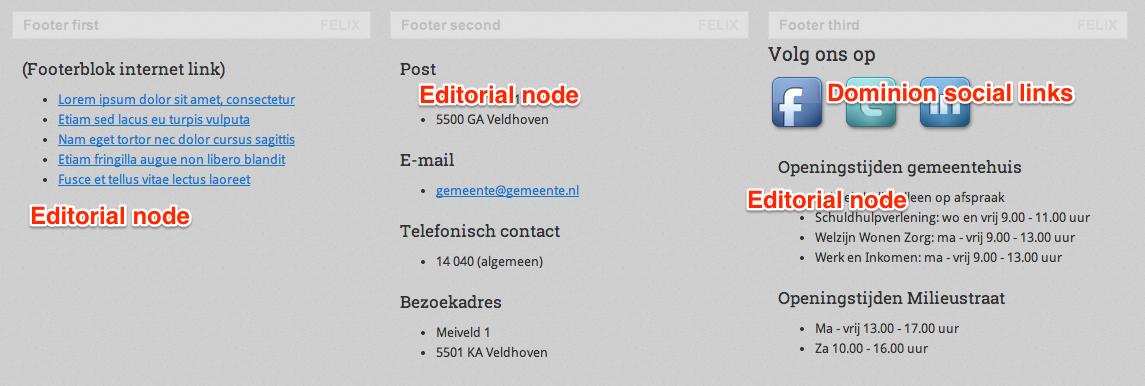
\includegraphics[width=\textwidth]{img/voorpagina3.png}
\end{center}
\subsection{Dashboard}\label{dashboard}
Het dashboard is de persoonlijke pagina voor ieder lid van het Intranet. Het is een pagina die is opgebouwd uit blokken die de gebruiker zelf kan aanzetten, uitzetten of verplaatsen.

In de onderstaande afbeelding zie je het Dashboard voor een Intranet gebruiker. 
Bij pijl 1 kun je blokken toevoegen aan je Dashboard. Elk blok heeft verschillende opties zoals inklappen, uitklappen en sluiten. Deze zijn te vinden bij pijl 2

\begin{center}
	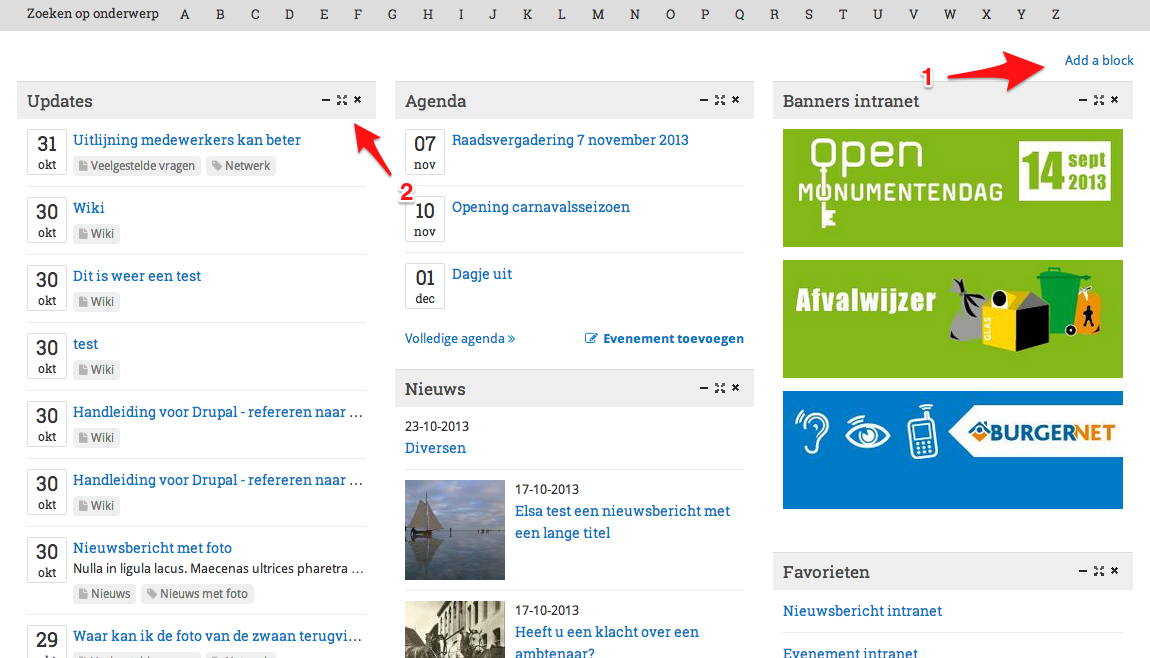
\includegraphics[width=\textwidth]{img/dashboard.png}
\end{center}

\subsection{Mobiel menu}

Op de mobiele versie verschijnt een blok met adres en telefoonnummer van het gemeentehuis. Dit blok is op een desktop browser ook te zien wanneer het scherm kleiner wordt gemaakt. Ingelogd als eindredacteur kan op deze manier ook de inhoud worden bewerkt op dezelfde manier als andere \emph{felix} blokken\seeone{felix}.
